\documentclass[12pt, a4paper]{article}
\usepackage[utf8]{inputenc}
\usepackage[T2A]{fontenc}
\usepackage{indentfirst, setspace}
\usepackage{tabularx, multirow}
\usepackage[normalem]{ulem}
\usepackage[style=russian]{csquotes}
\usepackage[english,russian]{babel}
\usepackage{hyperref}
\usepackage{ragged2e}
\usepackage{caption}
\usepackage{wrapfig}
\usepackage{amsmath}
\usepackage{tikz}
\makeatletter
\def\@biblabel#1{#1. }
\makeatother
\captionsetup{labelsep=endash}
\usepackage{listings}
\linespread{1.3}
\lstset{
  language=C++,
  basicstyle=\ttfamily\small,
  keywordstyle=\color{blue},
  breaklines=true,
  commentstyle=\color{green},
  stringstyle=\color{red},
  extendedchars=\true,
  showstringspaces=false,
  keepspaces=true,
}

\usepackage[left=2cm,right=2cm,
    top=2cm,bottom=2cm,bindingoffset=0cm]{geometry}\begin{document}
\begin{titlepage}
     \fontsize{12}{12}\selectfont

  {\centering

   \begin{bf}

    \begin{wrapfigure}{l}{10mm}
        
\includegraphics[width=17mm]{gerb3.2.jpeg}
    \end{wrapfigure}


    \noindent Министерство науки и высшего образования Российской Федерации

    \noindent Федеральное государственное бюджетное образовательное учреждение высшего образования

    \noindent \enquote{Московский государственный технический университет

     \noindent имени Н.Э. Баумана

     \noindent (национальный исследовательский университет)}

    \noindent (МГТУ им. Н.Э. Баумана)

   \end{bf}
  }

  \vspace{0.4cm}

  {\setstretch{0.1}
   \noindent\rule{\textwidth}{1mm}
   \noindent\rule{\textwidth}{0.5mm}

  }

  \fontsize{14}{21}\selectfont

  \noindent\begin{tabularx}{\textwidth}{l >{\centering\arraybackslash}X}
   ФАКУЛЬТЕТ & \flqq Фундаментальные Науки\frqq \\ \cline{2-2}

   КАФЕДРА & ФН-12 \flqq Математическое моделирование\frqq \\ \cline{2-2}
  \end{tabularx}

  \vspace{1cm}


  \begin{center}
   \begin{bf}

    \fontsize{24}{36}\selectfont
    ОТЧЕТ

    \fontsize{20}{30}\selectfont
    ПО ЛАБОРАТОРНОЙ РАБОТЕ НА ТЕМУ:

    Обратная польская запись

   \end{bf}
  \end{center}

  \fontsize{14}{21}\selectfont
  \vspace{5cm}


  \noindent\begin{tabularx}{\textwidth}{ X >{\centering}p{4cm} p{1cm} c }
   Студент: & & & Мациевский И. М. \\ \cline{2-2} \cline{4-4}
   & \fontsize{10}{15}\selectfont дата, подпись & & \fontsize{10}{15}\selectfont Ф.И.О. \\
   Преподаватель: & & & Волкова Л. Л.\\ \cline{2-2} \cline{4-4}
   & \fontsize{10}{15}\selectfont дата, подпись & & \fontsize{10}{15}\selectfont Ф.И.О.
   \end{tabularx}

  \vspace{\fill}

  \begin{center}
   \it{Москва}, 2023
  \end{center}

  \thispagestyle{empty}
\end{titlepage}\newpage
\tableofcontents
\newpage
\section*{Введение}
\addcontentsline{toc}{section}{Введение}
\justifying
\textbf{Цель лабораторной работы}: разработать программу для вычисления 
значений функции с использованием обратной польской записи.

Для достижения поставленной цели требуется решить следующие \textbf{задачи}.
\begin{enumerate}
\item Описать две формы записи --- инфиксную и постфиксную.
\item Разработать алгоритм проверки введенной инфиксной записи.
\item Реализовать алгоритм перевода из инфиксной записи в постфиксную 
форму записи.
\item Составить таблицу значений функции, при заданных границах и шаге 
аргумента.
\item Выполнить тестирование реализации разработанных алгоритмов.
\end{enumerate}
\newpage
\section{Аналитическая часть}
\subsection{Инфиксная запись}
\textbf{Инфиксная запись ---} это традиционный и способ записи 
математических выражений, при котором операторы располагаются между 
операндами, как это привычно в математике. Например: $a+b$, где $a$ и 
$b$ --- операнды, а $+$ является оператором сложения.
Для явного указания порядка операций, в инфиксной 
записи используются скобки.
\subsection{Постфиксная запись}
\textbf{Постфиксная запись ---} также известна как обратная польская 
запись, способ записи математических выражений, при котором операторы 
следуют после своих операндов. В постфиксной записи порядок операндов и 
операторов определяет последовательность выполнения операций. Ниже
представлены примеры постфиксных выражений.
	\begin{enumerate}
		\item Инфиксная запись: $a+b$, постфиксная запись: $a$ $b+$.
		\item Инфиксная запись: $3*(4+5)$, постфиксная запись: $3$ $4$ 
		$5$ $+*$.
		\item Инфиксная запись: $8/(2+3)$, постфиксная запись: $8$ $2$ 
		$3$ $+/$.
	\end{enumerate}

Постфиксная запись имеет преимущество в том, что она не требует 
использования скобок для уточнения порядка операций, поскольку 
последовательность операторов определена и не зависит от приоритета 
операторов, вследствие чего она более удобно для обработки компьютером.
\newpage
\section{Конструкторская часть}
\subsection{Проверка валидности строки}
Перед тем, как переводить строку из инфиксной записи в постфиксную, 
нужно проверить корректно ли составлена эта строка.
\begin{enumerate}
	\item Совпадает ли количество открывающихся скобок с количеством 
	закрывающихся.
	\item Нет ли двух знаков операций подряд.
	\item Количество операторов должно быть на единицу меньше 
	количества операндов.
\end{enumerate}
Все эти проверки можно сделать с помощью одного прохода по строке, 
сохраняя баланс скобок в переменную, делая проверку соседних элементов 
на то, не являются ли они оба операторами, подсчитывая количество
операторов и операндов.
\subsection{Перевод в ОПЗ}
Для перевода выражения из инфиксной в постфиксную запись используется 
алгоритм, который просматривает каждый символ входной строки, двигаясь 
от начала до конца. При этом создается строка, где будут храниться 
результаты в постфиксной записи, а также реализуется стек для 
операторов.
Когда встречается число или переменная, они добавляются в строку 
постфиксной записи, и курсор смещается. Если встречается открывающая 
скобка, она помещается в стек, и курсор также смещается. Если 
встречается оператор, его приоритет сравнивается с операторами в стеке. 
Если текущий оператор имеет приоритет выше или равный оператору на 
вершине стека, он помещается в стек. Если приоритет ниже, из стека 
извлекаются операторы и добавляются в постфиксное выражение, пока не 
выполняется условие приоритета.
Если встречается закрывающая скобка, выполняется цикл извлечения 
операторов из стека и добавления их в постфиксное выражение до тех пор, 
пока не встретится открывающая скобка.
По завершении обработки всех символов входной строки, извлекаются все 
оставшиеся операторы из стека и добавляются в конец постфиксного
выражения.
\subsection{Подсчет значения функции в ОПЗ}
Для нахождения значения функции в ОПЗ нужно пройти по строке в ОПЗ по 
следующему алгоритму.
\begin{enumerate}
	\item Если встретилось число, добавить его в стек.
	\item Если встретился бинарный оператор, два последних значения 
	берутся из стека в обратном порядке, над ними проводится
	арифмитическая операция, ее результат записывается в вершины стека.
	\item Если встретился унарный оператора, в данном случае - унарный 
	минус, берётся последнее значение из стека и вычитается из нуля, 
	так как унарный минус является правосторонним оператором.
	\item Если встретилась функция, она применяется к вершине стека,
	ее значение записывается в вершину стека.
	\item Последнее значение, после отработки алгоритма, является 
	решением выражения.
\end{enumerate}
\subsection{Реализованные функции}
Ниже представлены функции и классы, реализованные в проекте.
\begin{enumerate}
	\item $Stack$ --- стек.
	\item $isFunc$ --- определение является ли элемент функцией от $x$.
	\item $isOp$ --- определение является ли элемент оператором.
	\item $isNum$ --- определение является ли элемент числом.
	\item $valid_inf$ --- проверка корректности введенной строки.
	\item $priority$ --- определение приоритета функции.
	\item $infToPost$ --- перевод из инфиксной записи в постфиксную.
	\item $calculatePost$ --- подсчет значения выражения в ОПЗ.
\end{enumerate}
\newpage
\section{Технологическая часть}
Для реализации выбран язык C++.
На листинге 1 представлена реализация программы
(Реализация~\ref{lst:label1})
\begin{lstlisting}[caption={Исходный код}, label={lst:label1}]
#include <iostream>
#include <string>
#include <fstream>
#include <vector>
#include <cstdlib>
#include <limits>
#include <locale>
#include <stack>

using namespace std;

const double PI = 3.141592653589793;

template<typename T>
#define SIZE 10
class Stack
{
    T *arr;
    int top;
    int capacity;
 
public:
    Stack(int size = SIZE);
    ~Stack();
 
    void push(T);
    void pop();
    T peek();
    int size();
    bool isEmpty();
    bool isFull();
};

template<typename T>
Stack<T>::Stack(int size)
{
    arr = new T[size];
    capacity = size;
    top = -1;
}
template<typename T>
Stack<T>::~Stack() {
    delete[] arr;
}

template<typename T>
void Stack<T>::push(T x)
{
    if (isFull())
    {
        cout << "Ошибка. Стек переполнен";
        return;
    }
    arr[++top] = x;
}

template<typename T>
void Stack<T>::pop()
{
    if (isEmpty())
    {
        cout << "Ошибка. Стек пуст";
        exit(EXIT_FAILURE);
    }
    arr[top--];
}

template<typename T>
T Stack<T>::peek()
{
    if (!isEmpty()) {
        return arr[top];
    }
    else {
        exit(EXIT_FAILURE);
    }
}

template<typename T>
int Stack<T>::size() {
    return top + 1;
}

template<typename T>
bool Stack<T>::isEmpty() {
    if (top == -1) {
        return true;
    }
    return false;
}

template<typename T>
bool Stack<T>::isFull() {
    if (top == capacity - 1) {
        return true;
    }
    return false;
}


bool isFunc(string& token) {
    return (token == "sin" or token == "ctg");
}

bool isOp(string &c) {
    return (c == "+" or c == "-" or c == "*" or c == "/" or c == "^" or c == "(" or c == ")");
}

bool isNum(const string& s) {
    for (char c : s) {
        if (!isdigit(c) and c != '.' and c != '-') {
            return false;
        }
    }
    return true;
}


bool valid_inf(string &inf) {
    int brackets = 0;
    for (int i = 0; i < inf.size(); i++) {
        if (i == 0 and inf[i] == '-') {
            inf.insert(0, "0 ");
        }
        if (i > 1 and inf[i] == '-' and inf[i - 2] == '(') {
            inf.insert(i , "0 ");
        }
        if (i > 1 and (inf[i] == '-' or inf[i] == '+' or inf[i] == '*' or inf[i] == '/')
            and (inf[i - 2] == '-' or inf[i - 2] == '+' or inf[i - 2] == '*' or inf[i - 2] == '/')) {
            cout << "Ошибка в валидности операторов" << endl << endl;
            return 0;
        }
        if (i > 1 and inf[i] == '-' and (inf[i - 2] == '/' or inf[i - 2] == '*')) {
            inf.insert(i + 4, ") ");
            inf.insert(i, "( 0 ");
        }
        if (inf[i] == '(') {
            brackets++;
        }
        else if(inf[i] == ')'){
            brackets--;
            if (brackets < 0) {
                cout << "Неправильно расставлены скобки" << endl << endl;
                return false;
            }
        }
    }
    if (brackets != 0) {
        cout << "Неправильно расставлены скобки" << endl << endl;
        return false;
    }
    int operators = 0, operands = 0;
    for (int i = 0; i < inf.size(); i++) {
        string check;
        while (i < inf.size() and inf[i] != ' ') {
            check += inf[i];
            i++;
        }
        if (isOp(check)) {
            operators++;
            continue;
        }
        else if (isFunc(check)) {
            operators++;
            continue;
        }
        else if (isNum(check)) {
            operands++;
            continue;
        }
        else if (check == "x") {
            operands++;
            continue;
        }
        else {
            cout << "Ошибка в валидности токенов" << endl << endl;
            return 0;
        }
    }
    if (operands - 1 != operators) {
        cout << "Ошибка в валидности операторов" << endl << endl;
        return 0;
    }
    return true;
}

int priority(char op) {
    if (op == 's' or op == 'c')
        return 4;
    else if (op == '^')
        return 3;
    else if (op == '*' or op == '/')
        return 2;
    else if (op == '+' or op == '-')
        return 1;
    else
        return -1;
}

string infToPost(const string& expression) {
    stack<char> operators;
    string postfix;

    for (char c : expression) {
        if (c == ' ' or c == 'i' or c == 'n' or c == 't'  or c == 'g') {
            continue;
        }
        if (c == '.') {
            postfix += c;
            continue;
        }
        if (c != 's' and c != 'c' and isalnum(c)) {
            postfix += c;
        }
        else if (c == '(') {
            operators.push(c);
        }
        else if (c == ')') {
            while (operators.size() > 0 and operators.top() != '(') {
                postfix += ' ';
                postfix += operators.top();
                if (operators.top() == 's') {
                    postfix += "in";
                }
                if (operators.top() == 'c') {
                    postfix += "tg";
                }
                operators.pop();
            }
            if (operators.size() > 0 and operators.top() == '(') {
                operators.pop();
            }
        }
        else {
            while (operators.size() > 0 and priority(c) <= priority(operators.top())) {
                postfix += ' ';
                postfix += operators.top();
                if (operators.top() == 's') {
                    postfix += "in";
                }
                if (operators.top() == 'c') {
                    postfix += "tg";
                }
                operators.pop();
            }
            if (c != 's' and c != 'c') {
                postfix += ' ';
            }
            operators.push(c);
        }
    }

    while (operators.size() > 0) {
        postfix += ' ';
        postfix += operators.top();
        operators.pop();
    }

    return postfix;
}

double calculatePost(const string& expression) {
    setlocale(0, "");
    stack<double> operands;

    for(int i = 0; i < expression.size(); i++){
        if (expression[i] == ' ') {
            continue;
        }
        if (expression[i] == '-' and isdigit(expression[i + 1])) {
            int num = expression[i + 1] - '0';
            operands.push(-num);
            i = i + 2;
            continue;
        }
        if (isdigit(expression[i])) {
            if (expression[i + 1] == '.') {
                string numm;
                while (expression[i] != ' ') {
                    numm += expression[i];
                    i++;
                }
                locale::global(std::locale("en_US.UTF-8"));
                double num = std::stof(numm);
                operands.push(num);
                continue;
            }
            operands.push(expression[i] - '0');
        }
        else if (expression[i] == '+' or expression[i] == '-' or expression[i] == '*' or expression[i] == '/' or expression[i] == '^') {
            double operand2 = operands.top();
            operands.pop();
            double operand1 = operands.top();
            operands.pop();
            double result = 0.0;

            switch (expression[i]) {
            case '+':
                result = operand1 + operand2;
                break;
            case '-':
                result = operand1 - operand2;
                break;
            case '*':
                result = operand1 * operand2;
                break;
            case '/':
                if (operand2 == 0) {
                    return numeric_limits<float>::infinity();
                }
                result = operand1 / operand2;
                break;
            case '^':
                if (operand1 < 0 and (operand2 < 1 and operand2 > 0)) {
                    cout << "Корень из отрицательного числа" << endl;
                    return numeric_limits<float>::infinity();
                    break;
                }
                result = pow(operand1, operand2);
                break;
            }

            operands.push(result);
        }
        else if (expression[i] == 's') {
            double operand = operands.top();
            operands.pop();
            operands.push(sin(operand));
        }
        else if (expression[i] == 'c') {
            double operand = operands.top();
            operands.pop();
            if (PI / 2 == operand) {
                return numeric_limits<float>::infinity();
                break;
            }
            if (operand == 0) {
                return numeric_limits<float>::infinity();
                break;
            }
            operands.push(1.0 / tan(operand));
        }
    }
    return operands.top();
}

int main() {
    setlocale(0, "");
    string infix;
    getline(cin, infix);
    if (infix == "") {
        cout << "Пустая строка";
        return 0;
    }
    if (!valid_inf(infix)) {
        return 0;
    }
    
    string postfix = infToPost(infix);
    cout << "Постфиксная запись: " << postfix << endl << endl;

    int xmin, xmax, h;
    cout << "Введите xmin: ";
    cin >> xmin;
    cout << "Введите xmax: ";
    cin >> xmax;
    cout << "Введите h: ";
    cin >> h;
    cout << endl;
    
    for (int i = xmin; i <= xmax; i = i + h) {
        string dubler = postfix;
        for (int j = 0; j < postfix.size(); j++) {
            if (postfix[j] == 'x') {
                dubler.replace(j, 1, to_string(i));
            }
        }
        if (calculatePost(dubler) == numeric_limits<float>::infinity()) {
            cout << "x = " << i << "   f(x) = " << "---" << endl;
        }
        else {
            cout << "x = " << i << "   f(x) = " << calculatePost(dubler) << endl;
        }
        if (i + h > xmax and i < xmax) {
            for (int j = 0; j < postfix.size(); j++) {
                if (postfix[j] == 'x') {
                    dubler.replace(j, 1, to_string(xmax));
                }
            }
            if (calculatePost(dubler) == std::numeric_limits<float>::infinity()) {
                cout << "x = " << xmax << "   f(x) = " << "---" << endl;
            }
            else {
                cout << "x = " << xmax << "   f(x) = " << calculatePost(dubler) << endl;
            }
        }
    }

    return 0;
}
\end{lstlisting}
\newpage
На рисунках 1---9 представлены \textbf{примеры работы} описаннных выше 
алгоритмов.
\begin{enumerate}
	\item Входные файлы: корректная строка в инфиксной записи.\\
	Вывод программы --- ее постфиксная запись и значения. Результат 
	приведён на рис.~\ref{img:grap1}.
	\begin{figure}[h]
  		\center{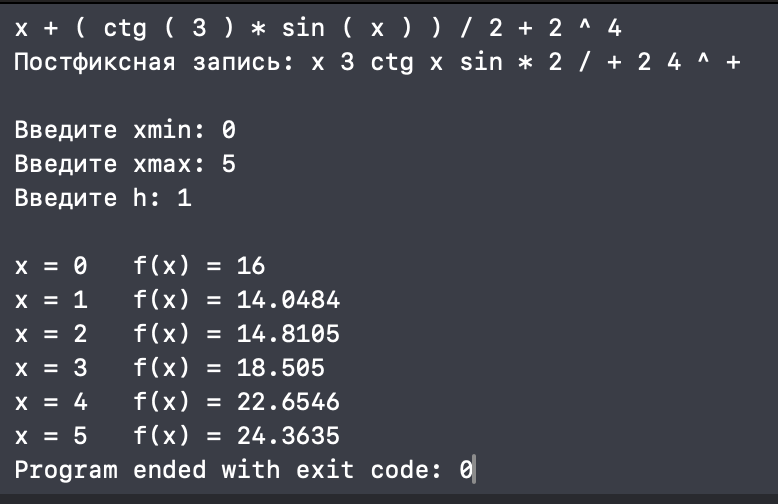
\includegraphics[scale=0.6]{ex10.png}}
  		\caption{Пример работы 1}
  		\label{img:grap1}
	\end{figure}
	\item Входные файлы: корректная строка в инфиксной записи.\\
	Вывод программы --- ее постфиксная запись и значения.
	Результат приведён на рис.~\ref{img:grap2}.
	\begin{figure}[h]
  		\center{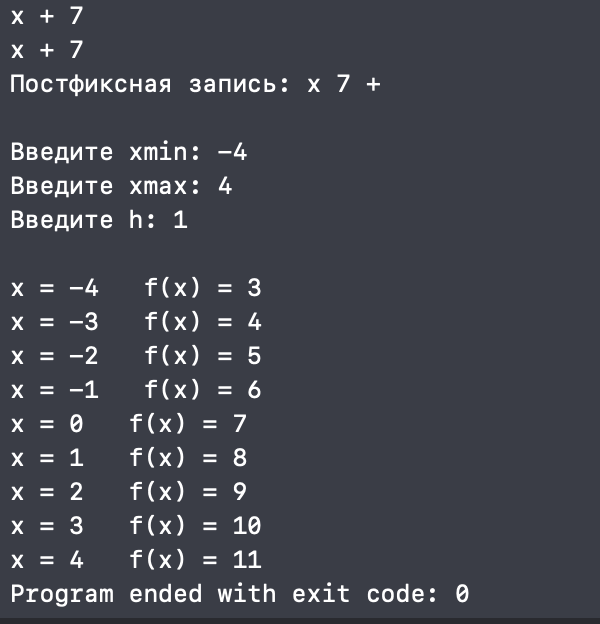
\includegraphics[scale=0.6]{ex1.png}}
  		\caption{Пример работы 2}
  		\label{img:grap2}
	\end{figure}
	\newpage
	\item Входные файлы: корректная строка в инфиксной записи.\\
	Вывод программы --- ее постфиксная запись и значения.
	Результат приведён на рис.~\ref{img:grap3}.
	\begin{figure}[h]
  		\center{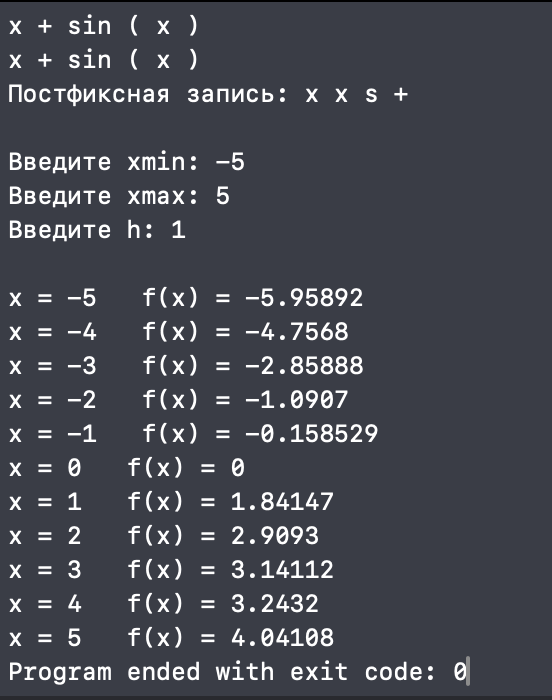
\includegraphics[scale=0.6]{ex3.png}}
  		\caption{Пример работы 3}
  		\label{img:grap3}
	\end{figure}
	\item Входные файлы: корректная строка в инфиксной записи.\\
	Вывод программы --- ее постфиксная запись и значения, причем в 
	точке 0 котангенс не определен, поэтому и значение функции не 
	определено в этой точке. Результат приведён на рис.~\ref{img:grap4}.
	\begin{figure}[h]
  		\center{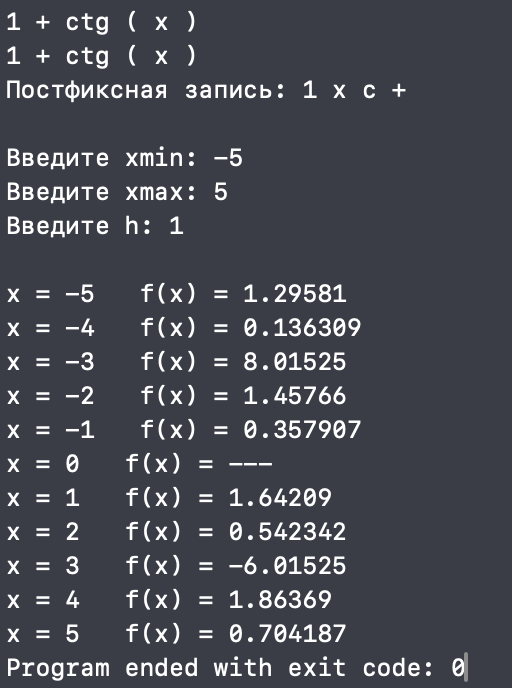
\includegraphics[scale=0.6]{ex2.png}}
  		\caption{Пример работы 4}
  		\label{img:grap4}
	\end{figure}
	\newpage
	\item Входные файлы: некорректная строка в инфиксной записи, два 
	знака подряд.\\
	Вывод программы --- ошибка. Результат приведён на 
	рис.~\ref{img:grap5}.
	\begin{figure}[h]
  		\center{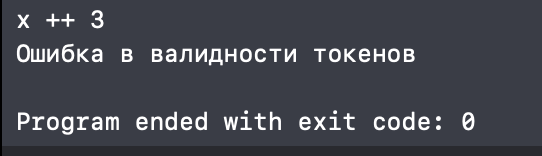
\includegraphics[scale=0.6]{ex4.png}}
  		\caption{Пример работы 5}
  		\label{img:grap5}
	\end{figure}
	\item Входные файлы: некорректная с математической точки зрения 
	строка, потому что котангенс 0 не определен.\\
	Вывод программы --- все значения функции тоже не будут определены.
	Результат приведён на рис.~\ref{img:grap6}.
	\begin{figure}[h]
  		\center{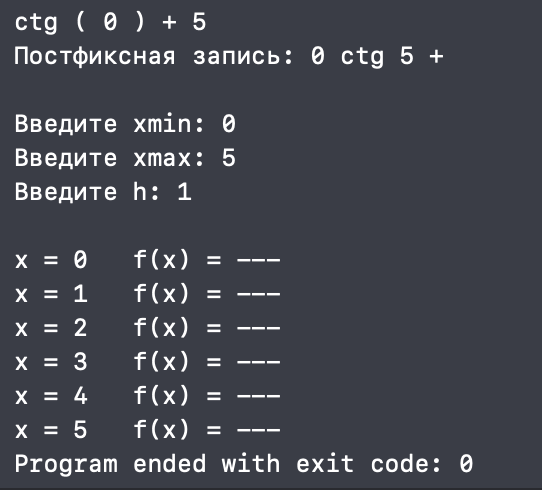
\includegraphics[scale=0.7]{ex5.png}}
  		\caption{Пример работы 6}
  		\label{img:grap6}
	\end{figure}
	\item Входные файлы: строка, в которой неверно расставлены скобки.\\
	Вывод программы --- ошибка. Результат 
	приведён на рис.~\ref{img:grap7}.
	\begin{figure}[h]
  		\center{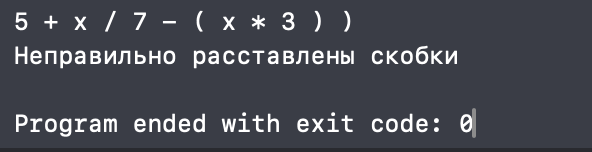
\includegraphics[scale=0.6]{ex6.png}}
  		\caption{Пример работы 7}
  		\label{img:grap7}
	\end{figure}
	\newpage
	\item Входные файлы: строка, в которой квадратный корень
	берется из отрицательного числа.\\
	Вывод программы --- ошибка. Результат 
	приведён на рис.~\ref{img:grap8}.
	\begin{figure}[h]
  		\center{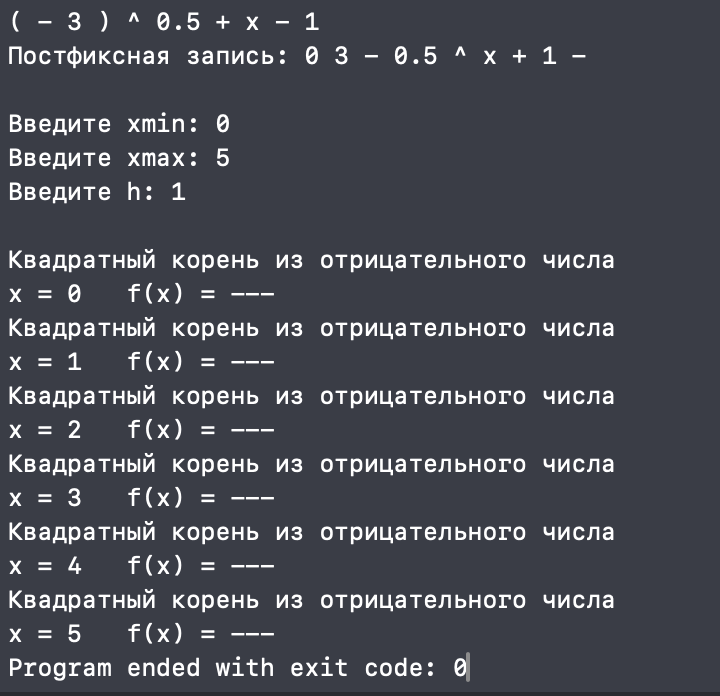
\includegraphics[scale=0.6]{ex7.png}}
  		\caption{Пример работы 8}
  		\label{img:grap8}
	\end{figure}
	\item Входные файлы: строка, в которой происходит
	деление на ноль.\\
	Вывод программы --- ошибка. Результат 
	приведён на рис.~\ref{img:grap9}.
	\begin{figure}[h]
  		\center{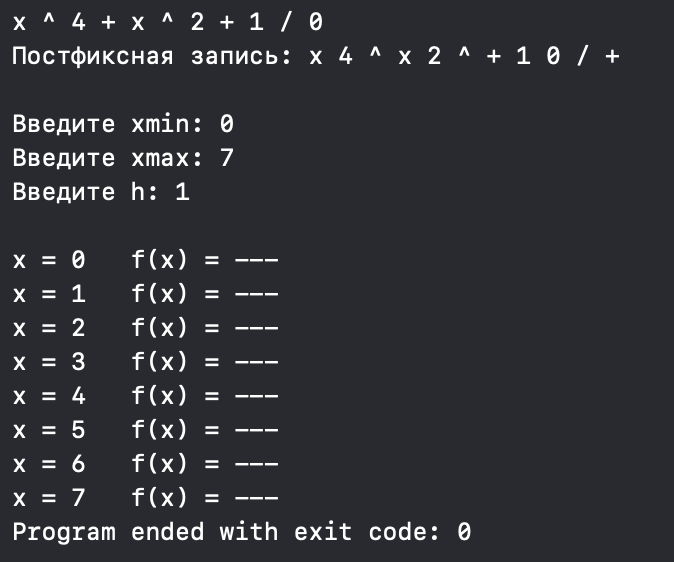
\includegraphics[scale=0.6]{ex8.png}}
  		\caption{Пример работы 9}
  		\label{img:grap9}
	\end{figure}
\end{enumerate}
\newpage
\section*{Заключение}
\addcontentsline{toc}{section}{Заключение}
Цель достигнута: разработана программа для вычисления значений функции 
с использованием ОПЗ и стека.
В результате выполнения лабораторной работы были выполнены все задачи.
\begin{enumerate}
	\item Описаны инфиксная и префиксная формы записи.
	\item Описан и реализован алгоритм перехода из инфиксной записи в 
	префиксную запись.
	\item Описан и реализован алгоритм поиска значения выражения в 
	инфиксной записи.
	\item Описан и реализован алгоритм проверки строки на корректность.
\end{enumerate}
\newpage
\begin{center}
\begin{thebibliography}{}
\addcontentsline{toc}{section}{Список используемых источников}
\bibitem{book}Фофанов О. Б., Алгоритмы и структуры данных: 
учебное пособие / Фофанов О. Б.; Томский политехнический университет. – 
Томск: Изд-во Томского политехнического университета, 2014. – 126 с.
\end{thebibliography}
\end{center}
\end{document}
